\newpage
%================================================================
\section{Results and Discussion}\label{sec:Results}
%================================================================

%----------------------------------------------------------------
\subsection{Validating the VMC Framework}\label{sec:project results}
%----------------------------------------------------------------

\autoref{fig:grid_search} shows the VMC computations of the expected energy and the corresponding variance with both the analytical and automatic differentiation approaches for a system of $N=1, 10, 100, 500$ non-interacting bosons in a spherical harmonic oscillator. We here use a grid search for the optimal variational parameter which is computationally expensive and generally infeasible for a non-coarse grid. However, in this case where we know the exact values, a grid search with a grid containing the exact value can be used to validate the sampling approach and implementation. As can be seen in the figure, the exact energy $\expval{E}/N = 3/2 \, \hbar \omega_\mathrm{ho}$ with $\Var \qty(E) / N = 0$ at $\alpha=1/2$ are found by both approaches, which indicates that the sampler works well and the implementation of the system is correct. The figure also illustrates the convex nature of the variational parameter optimization problem. In this study we optimize the variational parameter with respect to the expectation value of the energy, as described in \autoref{sec:gradient_descent}. However, the figure indicates that the variance might be more optimal as the optimization target since it tends to yield rather large values for non-optimal variational parameter values. 

\begin{figure}[!htb]
\centering
\subfloat[]{{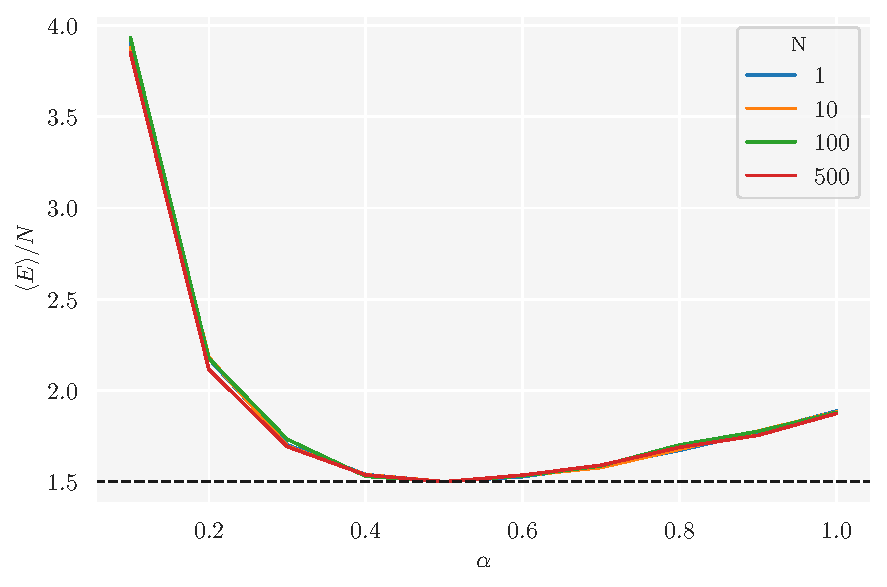
\includegraphics[width=0.47\textwidth]{latex/figures/grid_search_ashonib_rwm_energy.pdf}}}
\qquad
\subfloat[]{{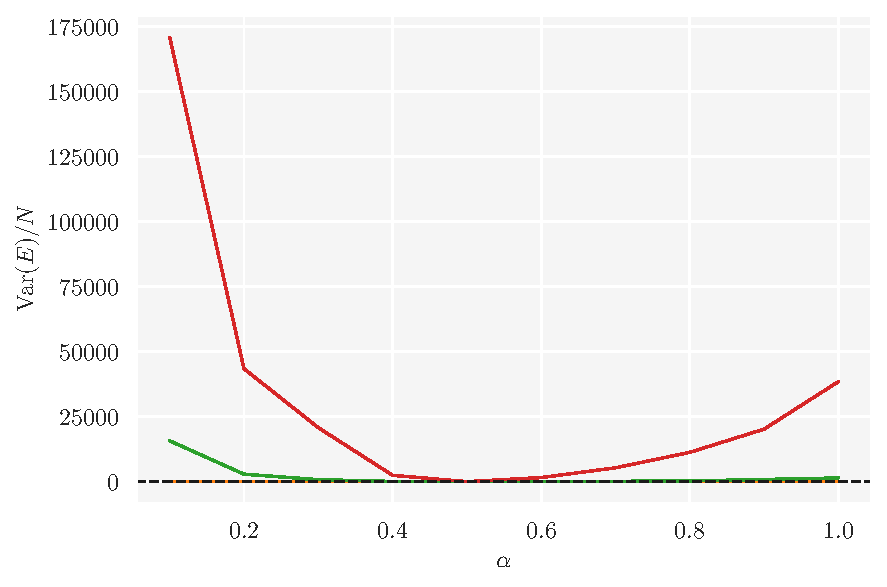
\includegraphics[width=0.47\textwidth]{latex/figures/grid_search_ashonib_rwm_variance.pdf}}}
\qquad
\subfloat[]{{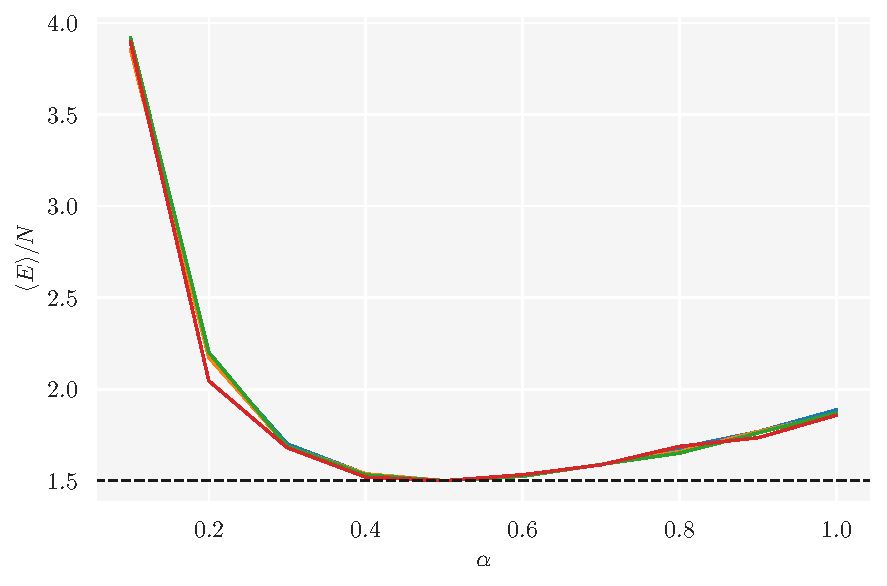
\includegraphics[width=0.47\textwidth]{latex/figures/grid_search_shonib_rwm_energy.pdf}}}
\qquad
\subfloat[]{{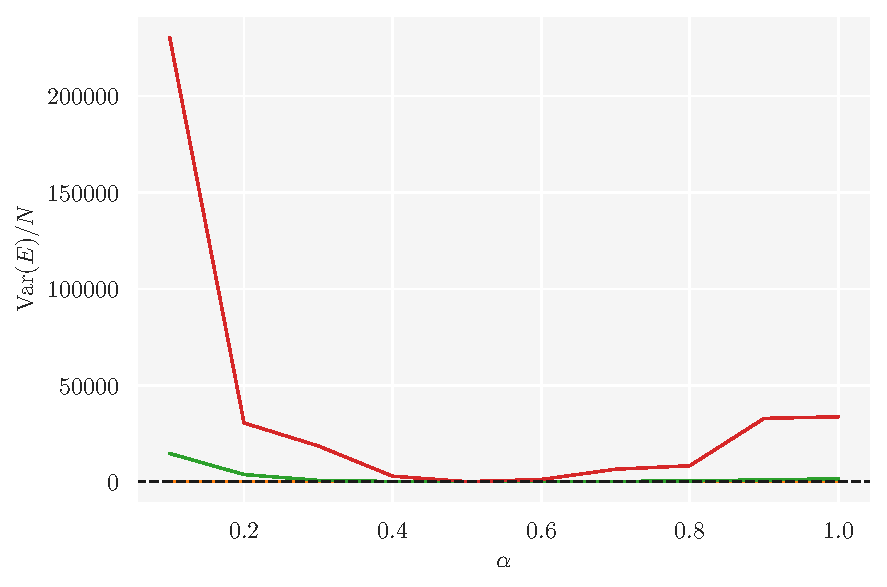
\includegraphics[width=0.47\textwidth]{latex/figures/grid_search_shonib_rwm_variance.pdf}}}
\caption{The expected value of the energy, $\expval{E}$, and variance, $\Var \qty(E)$, scaled  by the number of bosons, $N$, in a grid search for the optimal variational parameter $\alpha$. The system is a spherical harmonic oscillator with non-interacting bosons and the grid of variational parameters $\alpha \in [0.1, 1.0]$ with step size $0.1$. In \textbf{(a)} and \textbf{(b)} the expectation values are computed with the closed-form expressions, whereas in \textbf{(c)} and \textbf{(d)} the computations are done with automatic differentiation through JAX. Each computed point in the grid is the average over 16 tuned Markov chains with $20,000$ energy samples used to calculate the expectation values in each.}
\label{fig:grid_search}
\end{figure}




\autoref{tab:verification_energy} tabulates the computed expectation values of the energy using the same spatial configuration of interacting bosons in a spherical harmonic oscillator with two different implementations. One implementation is based on closed-form expressions in the linear domain whereas the other on closed-form expressions in the logarithmic domain (see \autoref{sec:analytical_interact}). As can be seen in the table, the expected energy calculations are identical for a given system size. As the implemented closed-form expressions found by different routes are identical, this further indicates the validity of the implementation.

\begin{table}[!htb]
\caption{Comparison between the implementation of analytical expressions for a system of interacting of bosons in a spherical harmonic oscillator. One is performed in the linear domain and the other in the log domain.}
\centering
\rowcolors{2}{gray!25}{white}
\begin{tabular}{ccc}
\hline
\hline 
\# of bosons & $\expval{E}$ linear domain & $\expval{E}$ log domain
\\
\hline 
\hline 
                   2 &         3.001 &                    3.001 \\
                   5 &         7.512 &                    7.512 \\
                  10 &        15.052 &                   15.052 \\
                  20 &        30.236 &                   30.236 \\
                  50 &        76.497 &                   76.497 \\
                 100 &       155.915 &                  155.915 \\
                 200 &       324.771 &                  324.771 \\
                 500 &       897.372 &                  897.372 \\
                1000 &     2,095.517 &                2,095.517 \\
\hline
\end{tabular}
\label{tab:verification_energy}
\end{table}

\autoref{fig:trace_phase} shows the three phases of the sampler for both the RWM and LMH algorithms used on a system of $N=100$ bosons in a spherical trap both with and without interactions. First, the sampler tunes the proposal scale parameter by increasing or decreasing it according to a look-up table (see \cw{vmc/utils/sampler_utils.py} in the source code) that tries to achieve a target acceptance rate. Then, the sampler search for the optimal variational parameter by employing gradient descent optimization, specifically, the ADAM optimizer discussed in \autoref{sec:adam}. The updates in the tuning and optimization phases are done after a set interval of MCMC steps. Both the tuning and optimization phase also employs early stopping, i.e., the phase will end if there is no change in values within a specified tolerance level between consecutive tuning or optimization intervals. Finally, the energy is sampled in what is hopefully the stationary state of the Markov chain. As can be seen in the figure, the different Markov chains all seem to converge well towards a stationary state by the time the sampler reaches the sampling phase. 

\begin{figure}[!htb]
\centering
\subfloat[]{{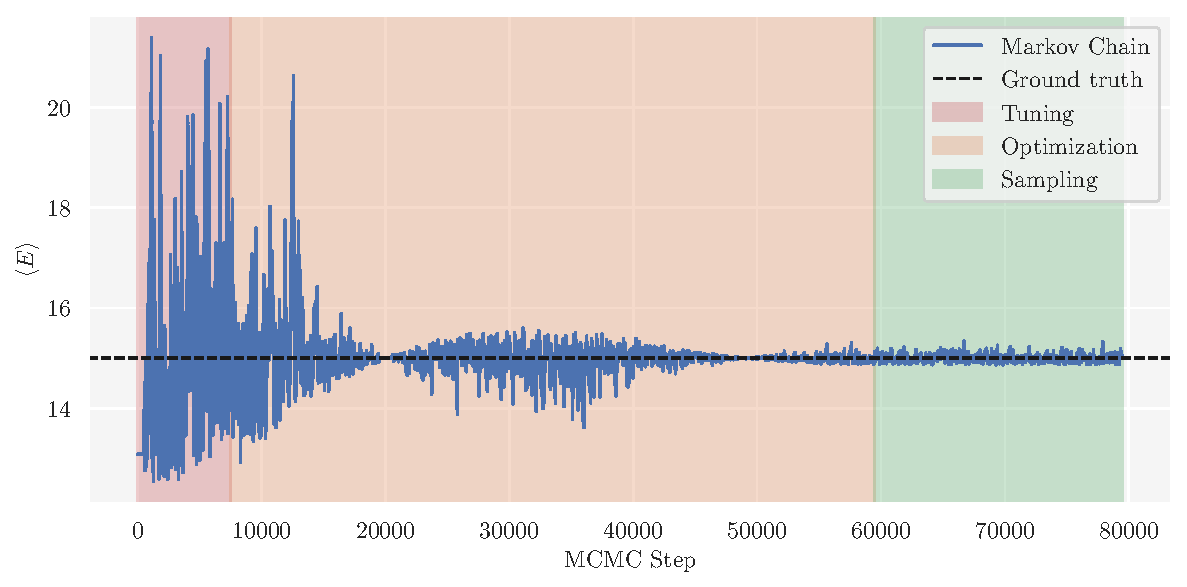
\includegraphics[width=0.47\textwidth]{latex/figures/trace_phase_rwm_ashonib.pdf}}}
\qquad
\subfloat[]{{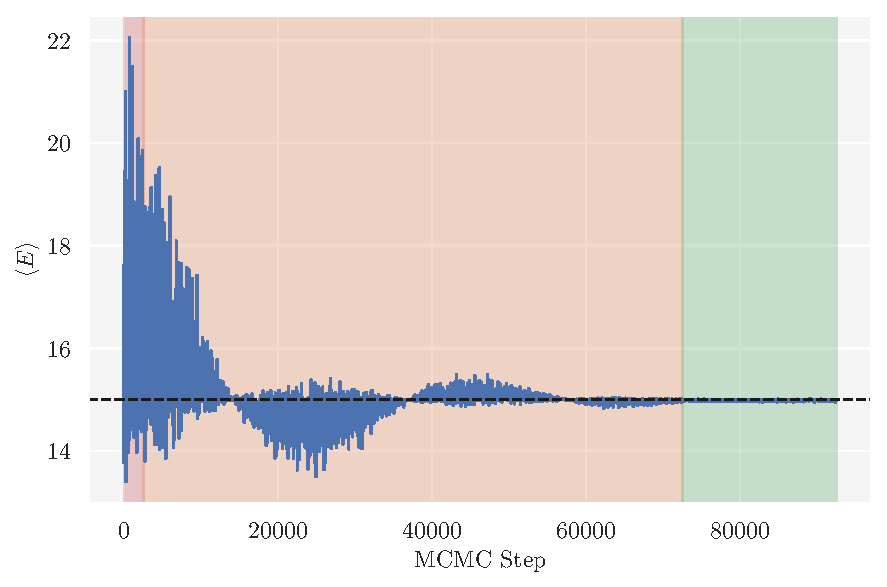
\includegraphics[width=0.47\textwidth]{latex/figures/trace_phase_lmh_ashonib.pdf}}}
\qquad
\subfloat[]{{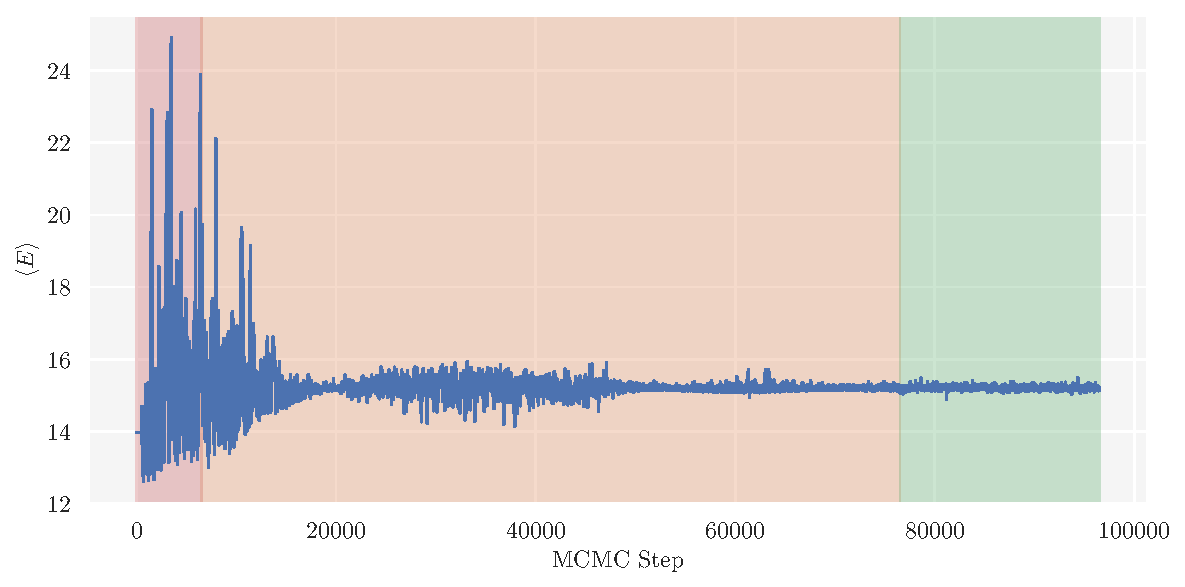
\includegraphics[width=0.47\textwidth]{latex/figures/trace_phase_rwm_ashoib.pdf}}}
\qquad
\subfloat[]{{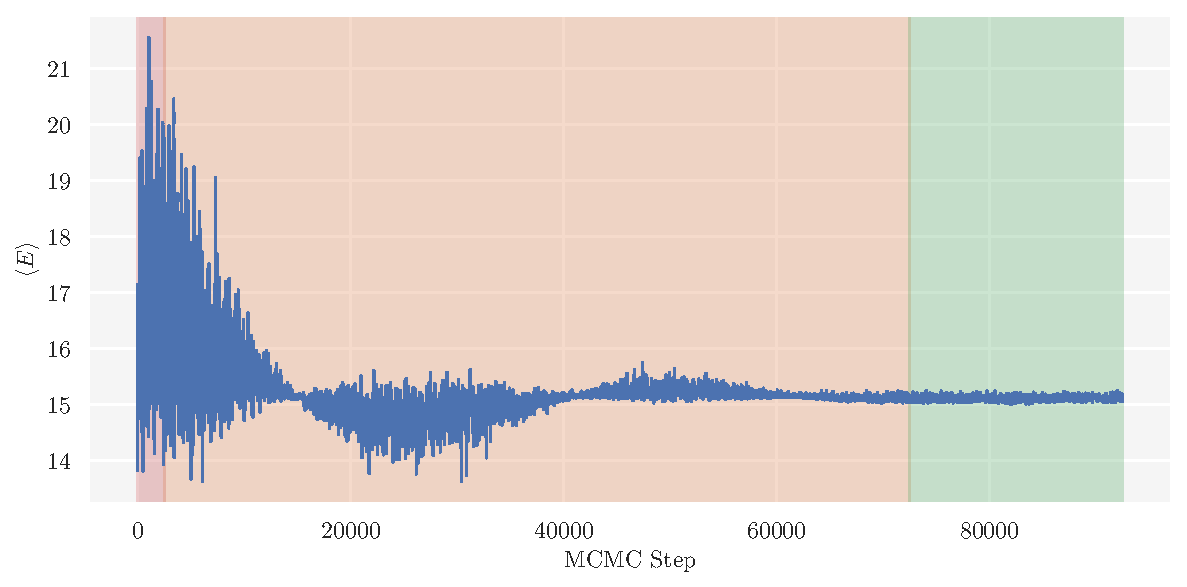
\includegraphics[width=0.47\textwidth]{latex/figures/trace_phase_lmh_ashoib.pdf}}}
\caption{The time evolution of a Markov chain in the three phases of the sampler; (i) tuning of the proposal scale parameter; (ii) gradient descent optimization of the variational parameter; and (iii) sampling of the variational energy. The updates in the tuning and optimization phase are done on a batch of samples, here 500 for tuning and 1000 for optimization. If the updated value remains the same between consecutive batches, the sampler will end the phase early. Here, the system consists of $N=100$ bosons in a spherical harmonic oscillator both with and without interactions. The initial variational parameter is set to $\alpha_0 = 0.4$. In \textbf{(a)} and \textbf{(b)} we see the RWM and LMH algorithm on a system of non-interacting bosons, respectively. In \textbf{(c)} and \textbf{(d)} we see the RWM and LMH algorithm on a system of interacting bosons, respectively.}
\label{fig:trace_phase}
\end{figure}

\FloatBarrier

%----------------------------------------------------------------
\subsection{Comparing the RWM and LMH algorithms}
%----------------------------------------------------------------

\autoref{fig:rwm_vs_lmh} shows the average energies, average statistical error and the variance in the energy, against the number of samples, $M$, for the RWM and LMH sampling algorithms on a spherically symmetric harmonic oscillator system of $100$ particles. The average energy per particle over $16$ chains is close to the exact energy for both the RWM and LMH samplers. The statistical error per particle in the RWM chains are almost a factor of $10$ larger than for the LMH chains, and the variance in the energy per particle shows that there are much larger fluctuations in the energy using the RWM than the LMH. 

This indicates that guiding the proposals according to the gradient flow of the probability density of the trial wave function, in fact does increase the sampling quality by a factor. 



%info: ASHONIB, $N=100$ particles, $10,000$ tuning cycles, $50,000$ optimization cycles, no early stopping, sampling cycles $M$, 16 chains, same $\alpha_0 = 0.4.$. Solid line is average over the 16 chains, shaded region the standard deviation of the mean (SEM). Statistical error estimated via blocking denoted $\sigma_B$. Used both RMW and LMH.

\begin{figure}[!htb]
\begin{center}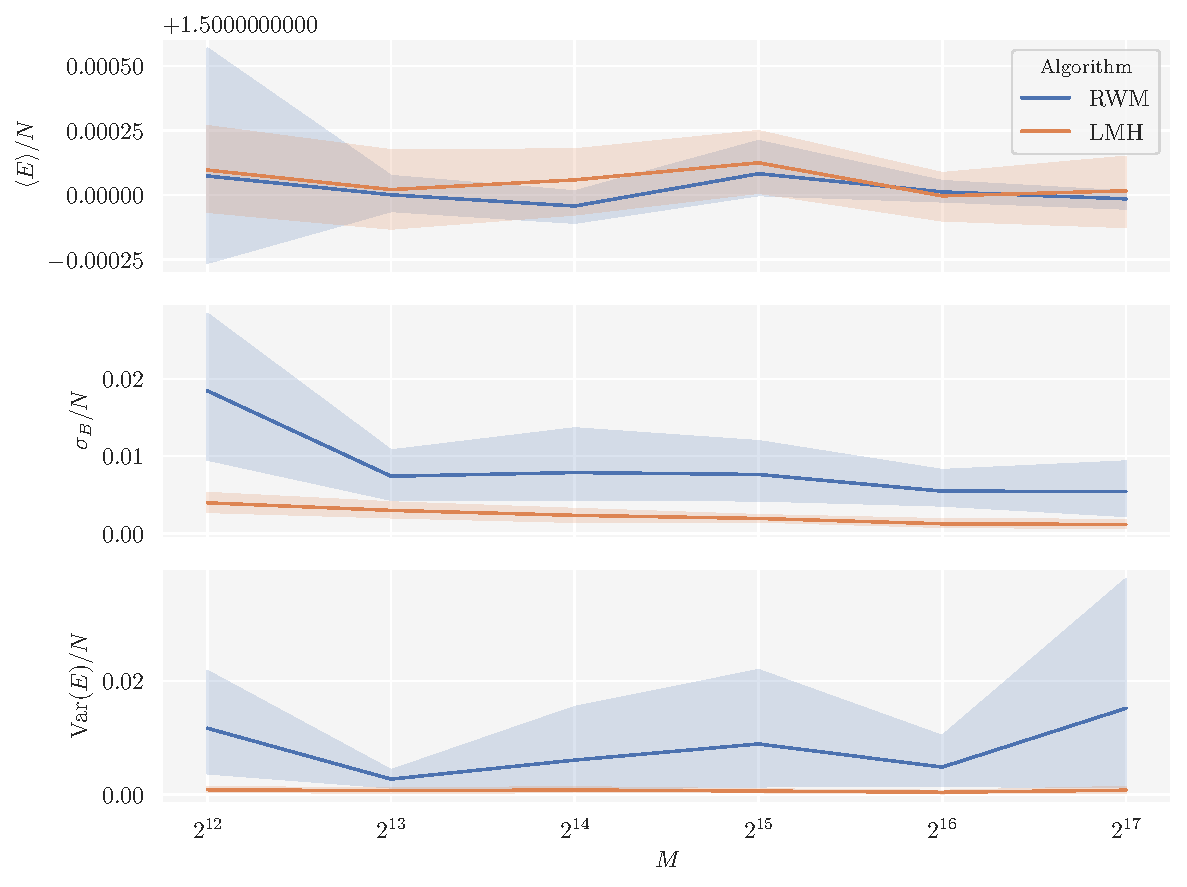
\includegraphics[width=\textwidth]{latex/figures/ashonib_N100_rwm_vs_lmh.pdf}
\end{center}
\caption{The sampled expected energy per particle ($\expval{E}/N$), the standard error ($\sigma_B/N$) and the variance ($\mathrm{Var}\qty(E)/N$) against the number of samples, $M$. The system is a spherical harmonic oscillator, with an initial $\alpha$-value of $0.4$. For every MCMC-chain run ($16$ per $M$-value), there were $10,000$ tuning cycles, and $\alpha$ was optimized over $50,000$ cycles. The solid lines indicates the average expected value over the $16$ chains, while the shaded region denotes the standard error of the mean. The blue lines and regions displays the results from the RWM algorithm, while the orange lines shows the corresponding results from the LMH algorithm.}
\label{fig:rwm_vs_lmh}
\end{figure}


% N: savner enhet på y-aksen i runtime plott, burde stå: Runtime [s] 
% J: Fiksa. Legend var bedre på siden, selv om det ikke er samme stil som over. 

The non-interacting system performs simple calculations in a highly efficient manner as it is easy to vectorise the calculations. \autoref{fig:runtime_comparison} shows run times for $20000$ tune cycles, $50000$ optimization cycles and $2^{15}$ sampling cycles for the Random Walk Metropolis and Langevin Metropolis-Hastings sampling algorithms, and using the analytical and numerical wave functions. There were $10$ runs for every $N\in[1, 10, 50, 100, 500]$ for every different sampler, and the error bars display the standard deviation of the $10$ samples. Adding more particles to the system only slightly increases the sampling time. The RWM algorithm is faster than the LMH algorithm, and the numerical implementation is slower than the analytical wave function. It seems that for the analytical samplers the LMH seems to take a rough factor of 4 more time than its RWM counterpart, but for the numerical computations (which needs to numerically calculate the Green's function for every step) it was a factor between 6-8 longer run time for the LMH sampler. 

The two comparisons in \autoref{fig:rwm_vs_lmh} and \autoref{fig:runtime_comparison} show that the number of samples to achieve the same quality sampling is quite different between the two approaches, and the LMH sampling algorithm seems to be more effective, even with the compuational costs taken into account. 

\begin{figure}[!htb]
\begin{center}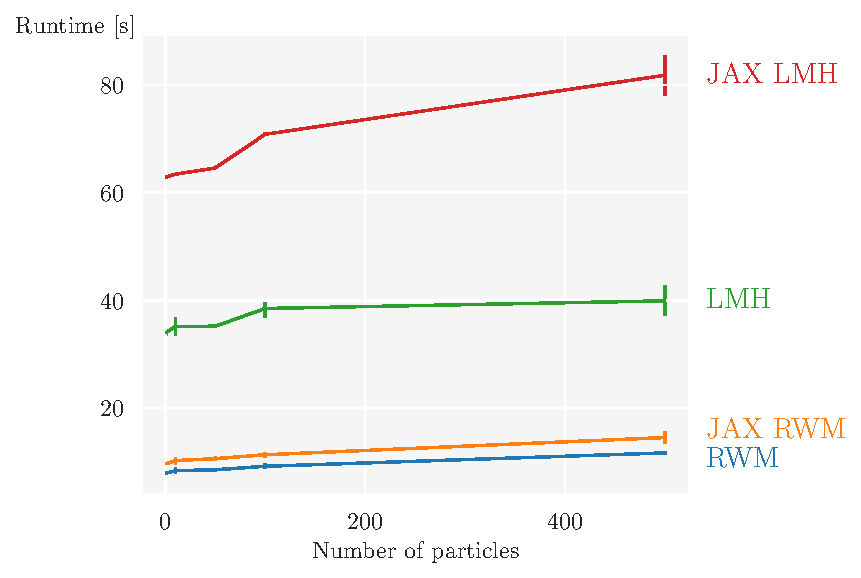
\includegraphics[width=\textwidth]{latex/figures/runtime_comparisons.pdf}
\end{center}
\caption{Runtimes for Random Walk metropolis and Langevin Metropolis-Hastings algorithms on spherical non-interacting systems with an analytical and numerical wave function (JAX). The error bars extend one standard deviation from the mean.}
\label{fig:runtime_comparison}
\end{figure}

%----------------------------------------------------------------
\subsection{Estimations of the Ground State Energy}
%----------------------------------------------------------------

Figure : RWM and LMH Spherical non-interacting / interacting (will go into appendix)

Figure: RWM LMH Elliptical non-interacting / interacting  
The elliptical potential described in \autoref{eq:Vtrap} yields a ground state energy per particle of $E_0/N = 2.414215 \hbar\omega_0$ for non-interacting particles. \autoref{fig:elliptical_energies} displays the mean energies and mean standard error (points), together with their spread (one standard error of the mean confidence interval)  of $16$ threads of sampling for each sampling algorithm. The parameters for the sampling runs were all set to a maximum of $20,000$ tuning cycles, with a tuning interval of $1000$. The initial alpha value was set to $0.5$ and the threads had all a maximum of $50,000$ optimization cycles, with an update at every $1,000$th cycle. The number of samples collected were $2^{15}$. 

\begin{figure}[!htb]
\centering
\subfloat[]{{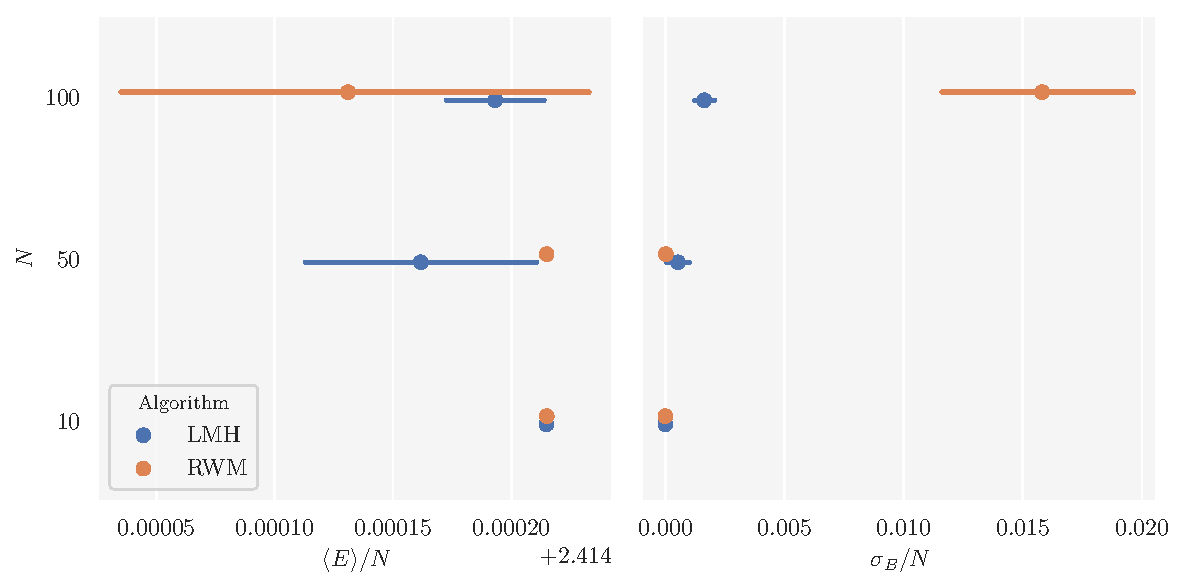
\includegraphics[scale=0.8]{latex/figures/non_interacting_elliptical_energies.pdf}}}
\qquad
\subfloat[]{{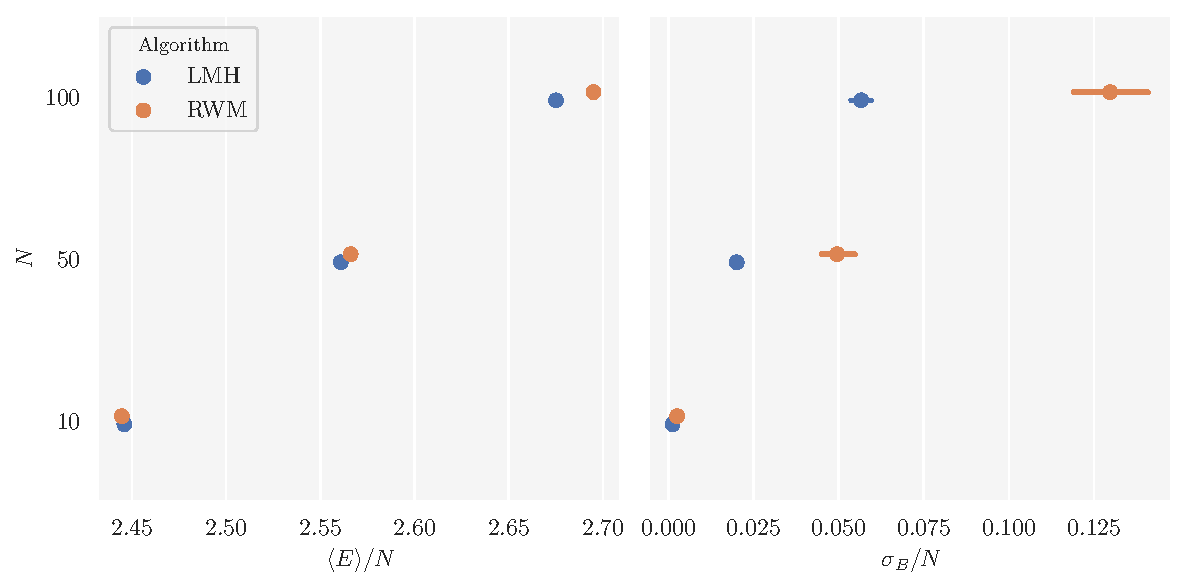
\includegraphics[scale=0.8]{latex/figures/interacting_elliptical_energies.pdf}}}
\caption{Sampled expected energies of the elliptical trap where the particles are non-interacting (\textbf{a}) and interacting (\textbf{b}). The sampled average energy per particle over $16$ chains against the number of particles are plotted to the left, and in the right windows the average statistical error per particle given by the blocking method is plotted. The stretch in the points shows spread in value by one standard error of the mean. The sample size is $M=2^{15}$, and there were a maximum of $20,000$ tuning cycles and $50,000$ optimization cycles, which could be less would the early stopping criterion be met.}
\label{fig:elliptical_energies}
\end{figure}

When the particles are interacting, the energy increases as a function of particle density in the trap. The collected mean energies together with the mean statistical error is tabulated in \autoref{tab:elliptical_energies}. The interacting bosons in the trap have a higher ground state than the non-interacting particles, and it increases with the number of particles. When the number of bosons in the trap increases, the density does too, meaning that the average distances to the nearest bosons decrease. Thus, we expect (and have seen in \citep{DuBois2001}) that the energy will continue to rise if we further increase the density. There is also the question of the quite large gap in average expected energies between the interacting systems when $N=100$ between the RWM and LMH sampling algorithms. This may have to do with the low number of samples produced by the chains, and the LMH algorithm has proven more effective in its choice of proposals. However, both values are well within one statistical error of each other, and may simply be due to the stochasticity of the procedures. 


\begin{table}[h]
\caption{Tabulated sampling results of $16$ sampling runs for each system and algorithm. The number of samples was $2^{15}$, with a maximum of $50,000$ optimization cycles and a maximum of $20,000$ tuning cycles. The system was a harmonic oscillator with an elliptical potential described by \autoref{eq:Vtrap}, with varying number of bosons. The hard-sphere diameter, $a$, is set to $0$ if there are no interactions between the bosons, while $a=a_{\mathrm{Rb}}=0.00433$ if the particles are interacting.}
\centering
\rowcolors{2}{gray!25}{white}
\begin{tabular}{ccccc}
\hline\hline
Measurement & LMH ($a=0$) & RWM ($a=0$) & LMH ($a=a_{Rb}$) & RWM ($a=a_{Rb}$)
\\
\hline \hline
$\expval{E}/(N=10)$[$\hbar\omega_0$] & 2.41421 & 2.41421 & 2.4459 & 2.4446  
\\
$\expval{E}/(N=50)$[$\hbar\omega_0$] & $2.4142$ & $2.4142$ & $2.5609$ & $2.5661$ 
\\
$\expval{E}/(N=100)$[$\hbar\omega_0$] & $2.4142$ & $2.4141$ & $2.6750$ & $2.6950$ 
\\
$\sigma_{\mathrm{B}}\qty(N=10)$[$\hbar\omega_0$] & $2\cdot10^{-7}$ & $3\cdot10^{-7}$ & $1\cdot10^{-3}$ & $3\cdot10^{-3}$ 
\\
$\sigma_{\mathrm{B}}\qty(N=50)$[$\hbar\omega_0$] & $5\cdot10^{-4}$ & $2\cdot10^{-5}$ & $2\cdot10^{-2}$ & $5\cdot10^{-2}$
\\
$\sigma_{\mathrm{B}}\qty(N=100)$[$\hbar\omega_0$] & $2\cdot10^{-3}$ & $2\cdot10^{-2}$ & $6\cdot10^{-2}$ & $1\cdot10^{-1}$
\\
\hline\hline
\end{tabular}
\label{tab:elliptical_energies}
\end{table}

%----------------------------------------------------------------
\subsection{One-Body Densities}
%----------------------------------------------------------------

\autoref{fig:one_body_densities} shows the sampled one-body densities for $10$ and $100$ particles in a spherical harmonic oscillator with the interactions turned on and off. As the number of particles increases, the density of particles increases, and the interactions between the particles become a larger factor. For $10$ particles, the one body densities with and without interactions are almost identical. This means that for $10$ particles, the interactions do not have a large impact on the system. For $100$ particles, the radial one body densities for the interacting and non-interacting cases differ more. The particles in the interacting case are more spread out in the $2$-dimensional space than the non-interacting case, which is expected, due to the repulsiveness of the Jastrow correlation factor. 
\begin{figure}[H]
\centering
\subfloat[]{{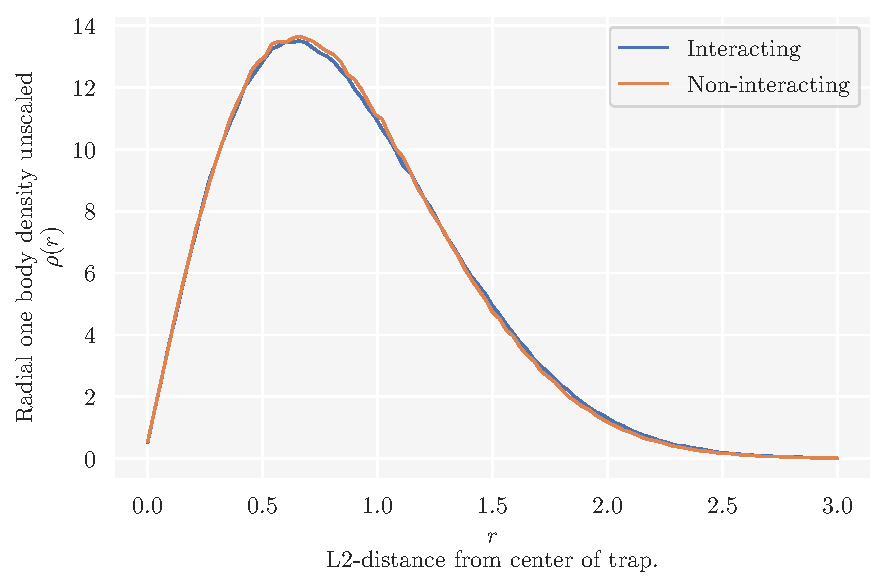
\includegraphics[width=0.47\textwidth]{latex/figures/OBD_N10.pdf}}} 
\qquad
\subfloat[]{{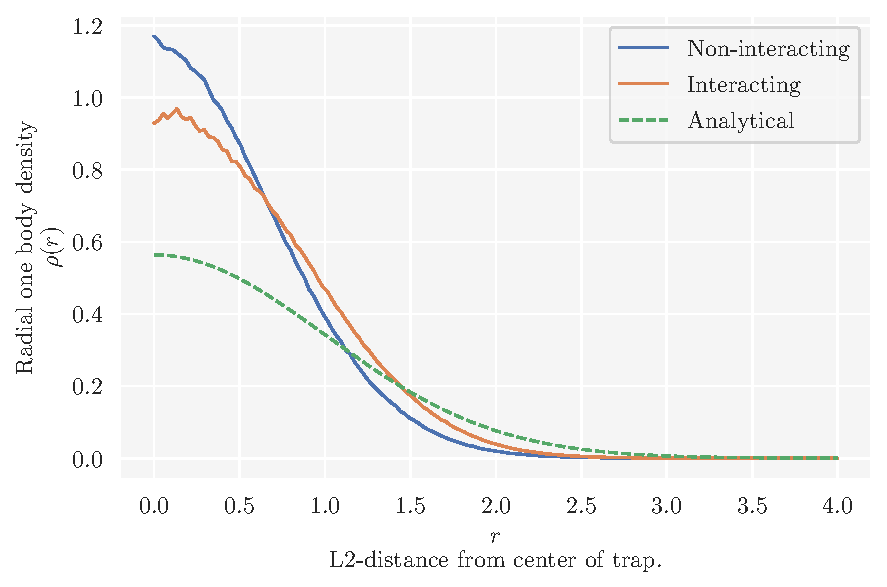
\includegraphics[width=0.47\textwidth]{latex/figures/OBD_N100.pdf}}}
\caption{\textbf{(a)} Comparison between the radial one body densities for $10$ particles with and without interactions (Jastrow factor $a=0.00433$) in $2$-dimensional space. \textbf{(b)} Comparison between the radial one body densities for $100$ particles with and without interactions (Jastrow factor $a=0.00433$) in $2$-dimensional space.}
\label{fig:one_body_densities}
\end{figure}



%%
%% N: Trenger vi noen av figurene under? Ekstra figurer kan gå i appendiks
%% J: Tror ikke det. Under variational energy, så har du kanskje kjørt optimize? 
% J: En annen ting, hvis du ser på y-aksen i OBD plots, og sammenligner med y-aksen i Figure 1 i DuBois, så er vår normalisert til å ha int_(space) = 1, mens deres er int_(space) = 0.5. Tror vi går for den vi har? 


%\subsubsection{One-body densities}

%\textbf{Elliptical potential}

%\autoref{fig:energy_elliptical} displays 16 independent energy sampling runs where $\alpha$ is optimized. 

%\begin{figure}[H]
%\begin{center}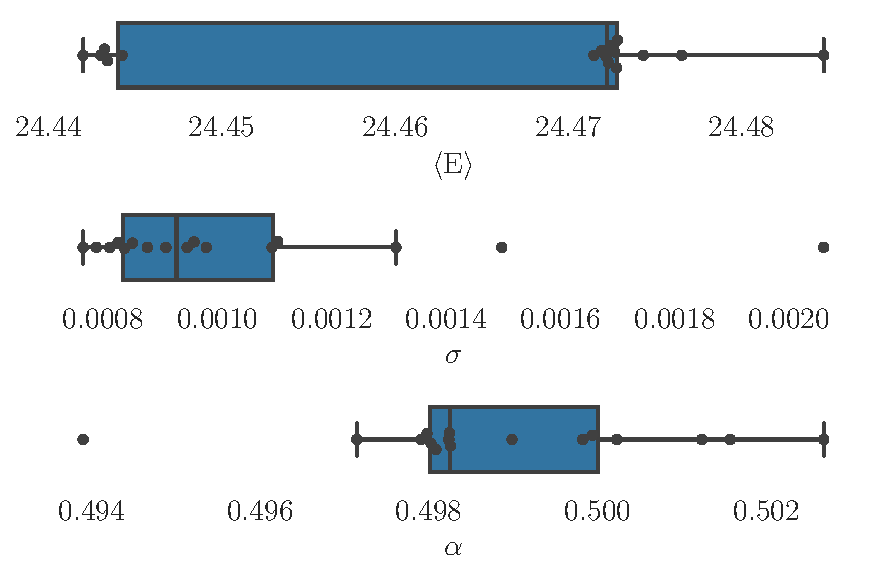
\includegraphics[scale=0.5]{latex/figures/aehoib_bp.pdf}
%\end{center}
%\caption{Sampled energies, the standard errors and the optimized $\alpha$-values of $16$ independent sampling runs.}
%\label{fig:bp_aehoib}
%\end{figure}

